\documentclass[a4paper, 11pt, twocolumn]{article}
\usepackage[margin=0.8in]{geometry}
\usepackage{xcolor}
\usepackage{graphicx} %package to manage images
\graphicspath{ {./images/} }

\title{A2-10 High Power Switching Systems}
\author{Revision sheet}
\date{}

\usepackage{fancyhdr}
\pagestyle{fancy}
\fancyhead{} % clear all header fields
\renewcommand{\headrulewidth}{0pt} % no line in header area
\fancyfoot{} % clear all footer fields
\renewcommand{\footrulewidth}{0.4pt}
\fancyfoot[C]{\thepage} % page number in centre of the page
\fancyfoot[R]{\footnotesize Thomas Boxall \\ Images from WJEC E-Book} % right hand footer has author name on top line and images reference on bottom line
\fancyfoot[L]{\footnotesize A2-10 High Power Switching Systems \\ Revision sheet} % left hand footer has title of document on top line and 'Revision Sheet' on bottom line


\begin{document}
    \maketitle

    \section{Introduction}
    \thispagestyle{fancy}
    Very high current loads require physically large switches. There are a few alternatives to using a giant switch.

    \section{DC Switching}
    There are a number of circuit designs which can be used to switch high current loads.
    \subsection{Relay Switch}
    There are a number of disadvantages to using a relay in this application. Relays are physical things which have contacts, these can become corroded or wear out. While the contact is closing, it can arc. Relays are physical electro-mechanical devices which can wear out.
    \subsection{Transistor Switch}
    These are an improvement over a relay as there are no physical components which can wear out, however the transistor still has problems. The transistors regions (cut off, linear and saturation) all have different voltage and current properties. The voltage and current are fine when the transistor is in cut off region or saturation region. This isn't the case in the linear region, current can flow through the device and there can be a voltage across it. This means power is dissipated and it gets hot.
    \subsection{Thyristor}
    This is a much better improvement over the transistor switch. \\
    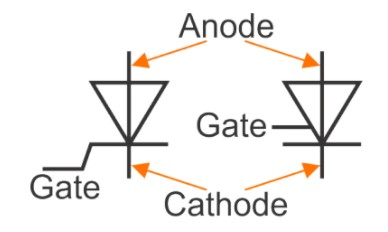
\includegraphics[width=0.4\textwidth]{thyristor.jpg}\\
    Current will only flow through the thyristor once the gate has been triggered with a sufficient current pulse. It is better than a relay because there are no moving parts to wear out and it is also faster, as again, there are no moving parts.
    \subsubsection{Conditions required for a Thyrsitor to conduct}
    \begin{itemize}
        \item Has to be in forward bias (anode is more positive than cathode)
        \item A sufficient pulse of current has been applied to the gate
        \item Sufficient load current flowing from anode to cathode (holding current)
    \end{itemize}
    \subsubsection{Key Quantities}
    $V_{GT}$ - Minimum gate voltage\\
    $I_{GT}$ - Minimum gate current\\
    $I_H$ - Holding current
    \subsubsection{Use of a Thyristor in a circuit}
    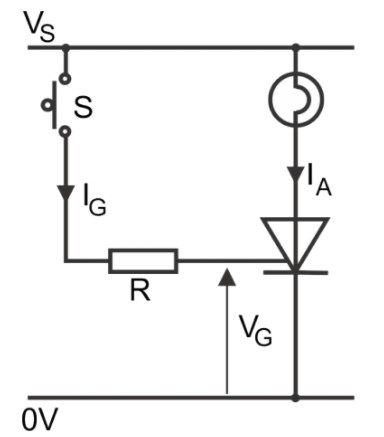
\includegraphics[width=0.4\textwidth]{thyristorCircuit1.jpg}
    \subsubsection{Thyristor transfer curve}
    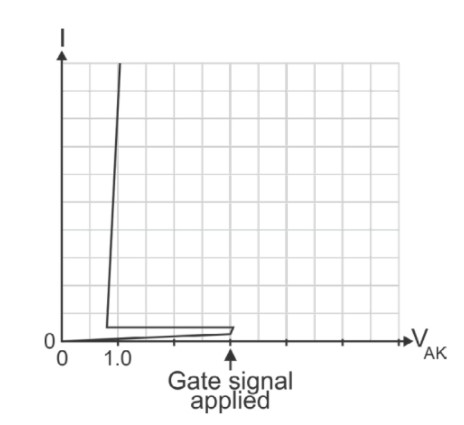
\includegraphics[width=0.4\textwidth]{thyristorGraph.jpg}\\
    When doing calculations with the thyristor, if it is switched off, there is no voltage across it.

    \subsection{Capacitor Commutation}
    It's great having a Thyristor to turn on the circuit, but what about when I want to turn it off. To do this, use capacitor commutation.\\
    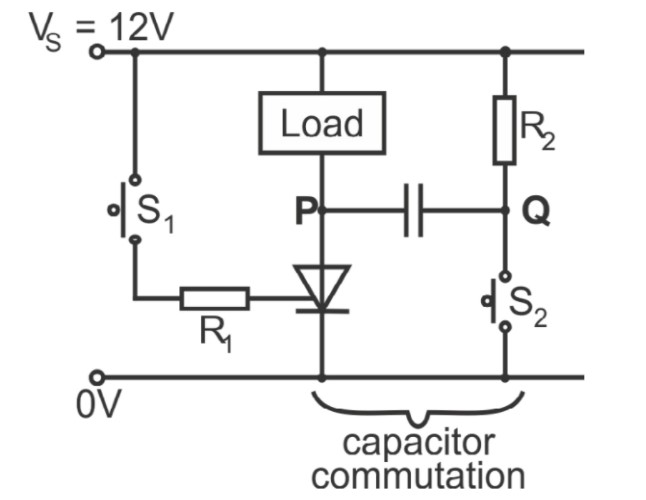
\includegraphics[width=0.4\textwidth]{capacitorCommutation.jpg}\\
    \begin{itemize}
        \item $S_1$ triggers Thyristor
        \item Before triggered: $V_P=+12V$, $V_Q=+12V$
        \item Once triggered: $V_P=0V$, $V_Q=+12V$, therefore C has 12V across it
        \item Press $S_2$, $V_Q=0V$ instantly
        \item C still has 12V across it. P must still be 12V below Q, therefore $V_P=-12V$
        \item Thyristor switches off as its now in reverse bias.
    \end{itemize}

    \section{RC Phase Shift}
    A resistor and capacitor connected in series can be used to take the output voltage from the RC subsystem out of phase with the input.\\
    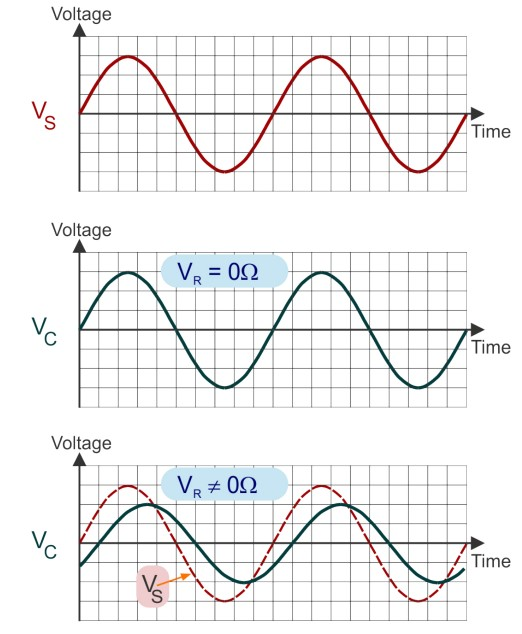
\includegraphics[width=0.4\textwidth]{phaseShift.jpg}\\
    Phase Shift is measured in degrees and has the symbol \o. Phase shift is between 0\textdegree and 90\textdegree and can be calculated with the following formula:\\
    \o $\displaystyle = \tan^{-1}\frac{R}{X_C}$

    \section{AC Switching}
    Thyristors can't be used for AC signals. If we did use a thyristor for an AC signal, it would look something like half wave rectification. We have to use a different component instead.
    \subsection{Triac}
    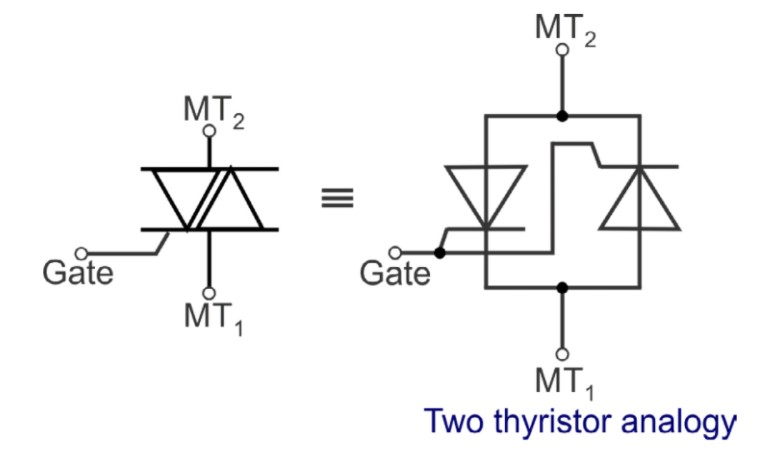
\includegraphics[width=0.4\textwidth]{triac.jpg}\\
    It can be triggered by a positive or negative pulse to the gate. It switches off when the voltage input crosses 0V until it is triggered again. Therefore it has to be triggered frequently (about 50 times per second) for a constant output.\newline
    We can combine the triac and phase shift subsystem together to give us the following circuit.\newline
    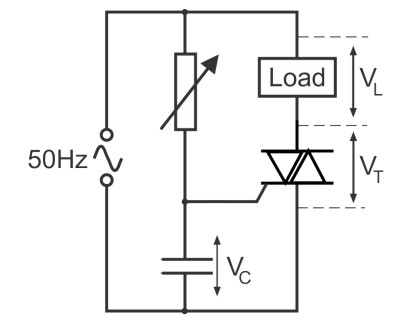
\includegraphics[width=0.4\textwidth]{triacAnd PhaseShift.jpg}\newline
    The triac is triggered by $V_C$, when $V_C$ reaches $V_{GT}$. As we have R, $V_C$ is out of phase with $V_S$ therefore the triac gets triggered at random points.\newline
    The more phase shift we have, the more the wave is 'chopped up', this results in less power in the load. This is very useful for controlling lights, heaters and motors (anything with a dimmer switch).\newline
    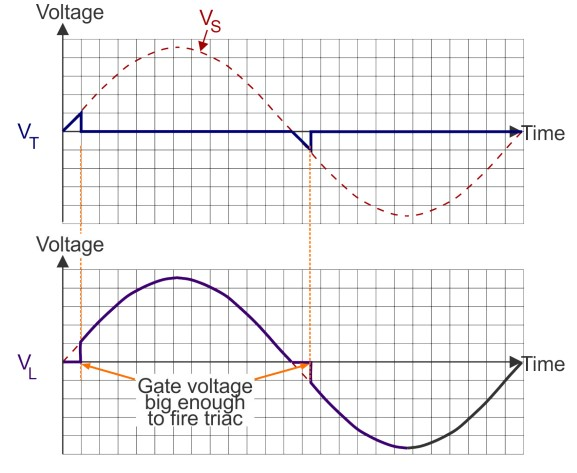
\includegraphics[width=0.4\textwidth]{triacOut.jpg}

    \subsection{Improvements To The Triac Circuit}
    There are a number of issues with the triac circuit, these are:
    \begin{itemize}
        \item $V_C$ varies slowly
        \item Gate voltage on the triac is vague. Therefore triggering isn't sharp therefore sometimes voltage and current through triac at the same time (this means power gets dissipated)
    \end{itemize}
    We can add a diac to the circuit to solve the problems.
    \subsection{Diac}
    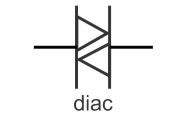
\includegraphics[width=0.4\textwidth]{diac.jpg}\\
    Diacs conduct voltage when it their input exceeds their breakover voltage. They switch on quickly, this can speed up phase control switching.\\
    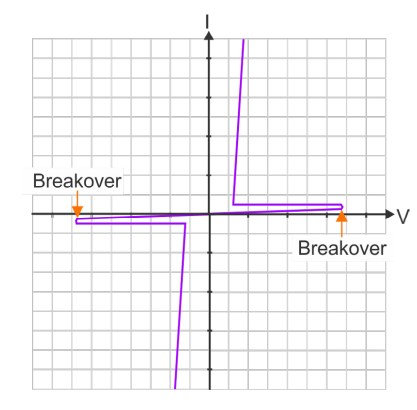
\includegraphics[width=0.4\textwidth]{diacGraph.jpg}\\
    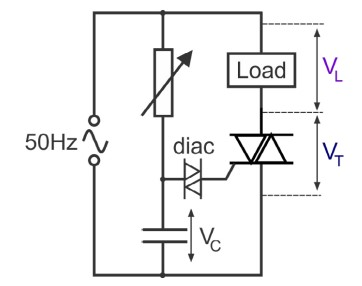
\includegraphics[width=0.4\textwidth]{diacCircuit.jpg}\\
    The diac will conduct when $V_C$ reaches the breakover voltage, then it will trigger the triac's gate quickly.\\
    Triac phase control circuits produce lots of noise. The Diac reduces the power dissipation in the triac.

\end{document}